\documentclass[UTF8]{ctexbook}

\usepackage[]{ctex}
\usepackage{amsmath}
\usepackage{geometry}
\usepackage[colorlinks=true]{hyperref}
\usepackage{indentfirst}
\usepackage[center]{titlesec}
\usepackage{graphicx}
\usepackage{esint}
\usepackage{cases}

\geometry{left=1cm,right=1cm,top=3cm,bottom=3cm}
\title{db的日常笔记}
\date{最后的编译日期:\today}
\author{dbydd}    
\kaishu
\setlength{\parindent}{2em}
\titleformat{\section}[block]{\LARGE\itshape\mdseries}{\arabic{section}}{1em}{}[]
\titleformat{\subsection}[block]{\Large\itshape\mdseries}{\arabic{section}.\arabic{subsection}}{1em}{}[]
\titleformat{\subsubsection}[block]{\large\itshape\mdseries}{\arabic{section}.\arabic{subsection}.\arabic{subsubsection}}{1em}{}[]
\titleformat{\paragraph}[block]{\small\bfseries}{[\arabic{paragraph}]}{1em}{}[]
\setcounter{secnumdepth}{3}
\setcounter{tocdepth}{3}

\newcommand{\limNormal}[1]{\lim\limits_{#1}}
\newcommand{\myLimToZero}{\limNormal{x \to 0}}
\newcommand{\myLimToInf}{\limNormal{x \to \infty}}
\newcommand{\derivative}{^\prime}
\newcommand{\doubleDerivative}{^{\prime\prime}}
\newcommand{\tripleDerivative}{^{\prime\prime\prime}}
\newcommand{\aLotDerivative}[1]{^{(#1)}}
\newcommand{\partialDerivative}[1]{^\prime_{#1}}
\newcommand{\myLeftRightArrow}{$\Leftrightarrow$}
\newcommand{\myRightArrow}{$\Rightarrow$}
\newcommand{\mathCombination}[2]{C_{#1}^{#2}}
\newcommand{\mathPermutation}[2]{P_{#1}^{#2}}
\newcommand{\upDownSum}[2]{\sum\limits_{#2}^{#1}}
\newcommand{\upDownProd}[2]{\prod\limits_{#2}^{#1}}
\newcommand{\fDerivative}[1]{\fint\derivative(#1)}
\newcommand{\defFunction}[1]{\fint(#1)}
\newcommand{\definiteIntegral}[2]{\int^{#1}_{#2}}
\newcommand{\mathConstant}{\mathbf{C}}
\newcommand{\degree}{^\circ}
\newcommand{\projection}[1]{Prj_{#1}}
\newcommand{\mathRealNumberCollection}{\mathbf{R}}


\begin{document}
\pagestyle{empty}{
  \maketitle
  \paragraph{todos}{
    \begin{enumerate}
      \item 誊录纸质笔记
      \item 空间解析几何\ 叉乘
      \item 给线性代数部分引入线性映射的观点。
      \item 补充多个section,计算机图形学,场论等
    \end{enumerate}
  }
  \tableofcontents
  \newpage
}
\setcounter{page}{1}
\chapter{数学}{
\section{基本概念}{
\subsection{六大基本初等函数}{
  常数函数,幂函数,指数函数,对数函数,三角函数
}%六大基本初等函数结尾

\subsection{介值定理}{
在数学分析中,介值定理(英语:intermediate value theorem,又称中间值定理)描述了连续函数在两点之间的连续性:

假设有一连续函数$\fint:[a,b]\rightarrow \mathbf{R}$, 且假设$\fint(a)<\fint(b)$, 若对任意数$u$满足$\fint(a)<u<\fint(b)$,则存在一点$c,a<c<b$,使得$\fint(c) = u$,当$\fint(a)>\fint(b)$时也有类似叙述

直观的比喻:这代表在$[a,b]$区间上可以画出一条连续曲线,而不让笔离开纸面。
\newline

定理:

假设$I = [a,b]$是一个实数里的闭区间,而$f:I\rightarrow\mathbf{R}$是连续函数,那么其像集$\fint(I)$也是区间。他或者包含$[\fint(a),\fint(b)]$(如果$\fint(b)\leq\fint(a)$)。换言之:

$\fint(I)\supseteq[\fint(a),\fint(b)]$。

或:

$\fint(I)\supseteq[\fint(b), \fint(a)]$。

介质定理通常以下述等价的形式表述:假设$f:I\rightarrow\mathbf{R}$是连续函数,且实数$u$满足$\fint(a)<u<\fint(b)$或$\fint(a)>u>\fint(b)$,则存在$c\in(a,b)$使得$\fint(c) = u$

图示:
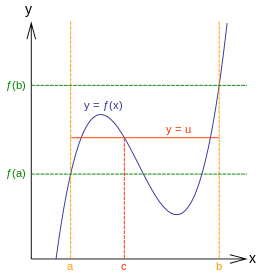
\includegraphics{resources/Intermediatevaluetheorem.png}
}%介值定理结尾

\subsection{二项式定理}{
  $(x + y)^n = x^n + \mathCombination{n - 1}{n}(x^{n-1} y) + \mathCombination{n - 2}{n}(x^{n-2} y^2) + \dots + y^n$
}%二项式定理结尾

\subsection{排列组合}{
  排列:$\mathPermutation{m}{n} = \frac{m!}{(m-n)!}$

  组合:$\mathCombination{m}{n} = \frac{\mathPermutation{m}{n}}{m!} = \frac{n!}{m!(n-m)!}$
}%排列组合结尾

\subsection{极坐标}{
极坐标是不同于笛卡尔坐标系(直角坐标系)的另一种函数图像平面。

极坐标不同于笛卡尔坐标系,他没有x和y轴,而是用基准轴和角度表示一个点。

\subsubsection{极坐标系下的面积}{
  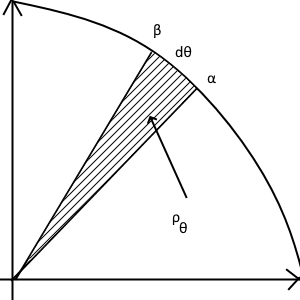
\includegraphics{resources/polar_coordness.png}

  公式为$\frac{1}{2}\definiteIntegral{\beta}{\alpha}(p(\theta))^2d\theta$

  p是形成曲线的函数。
  }%极坐标下的面积结尾

  \subsubsection{转换公式}{
    从笛卡尔坐标系到极坐标有一套转换公式。

    $$
      \begin{cases}
        x = \rho\cos\theta \\
        y = \rho\sin\theta
      \end{cases}
    $$
  }%转换公式结尾

}%极坐标结尾

\subsection{不等式}{

\subsubsection{基本不等式}{
  $\frac{a + b}{2} \geq \sqrt{ab}$

  注:当且仅当$a = b$时取等号

  其中$\frac{a+b}{2}$称为$a,b$的算数平均数,$\sqrt{ab}$称为$a,b$的几何平均数。

  将其变形,可得:
  \begin{enumerate}
    \item $a + b \geq 2\sqrt{ab}$(当且仅当$a = b$时取等号)
    \item $\frac{b}{a} + \frac{a}{b} \geq 2$($a,b$同号)
    \item $ab \leq (\frac{a + b}{2})^2$($a,b\in\mathRealNumberCollection$)
    \item $(\frac{a + b}{2})^2 \leq \frac{a^2 + b^2}{2}$($a,b\in\mathRealNumberCollection$)
  \end{enumerate}
}%基本不等式结尾

\subsubsection{均值不等式}{
平均数不等式,或称平均值不等式、均值不等式,是数学上的一组不等式,也是基本不等式的推广。它是说:

如果$x_{1},x_{2},\dotsm,x_{n}$是正数,则:

$\mathbf{H}_n \leq \mathbf{G}_n \leq \mathbf{A}_n \leq \mathbf{Q}_n$

其中:

$\mathbf{H}_n = \frac{n}{\upDownSum{n}{i = 1}\frac{1}{x_i}} = \frac{n}{\frac{1}{x_1} + \frac{1}{x_2} + \dotsm + \frac{1}{x_n}}$

$\mathbf{G}_n = \sqrt[n]{\upDownProd{n}{i = 1}x_i} = \sqrt[n]{x_1x_2\dotsm x_n}$

$\mathbf{A}_n = \frac{\upDownSum{n}{i = 1}x_i}{n} = \frac{x_1 + x_2 + x_n}{n}$

$\mathbf{Q}_n = \sqrt{\frac{\upDownSum{n}{i = 1}x^2_i}{n}} = \sqrt{\frac{x^2_1 + x^2_2 + \dotsm + x^2_n}{n}}$

当且仅当$x_1 = x_2 = \dotsm = x_n$,等号成立。

当$n = 2$时:

$\frac{2}{\frac{1}{x_1} + \frac{1}{x_2}} = \frac{2x_1x_2}{x_1 + x_2}\leq\sqrt{x_1x_2}\leq\frac{x_1 + x_2}{2}\leq\sqrt{\frac{x_1^2 + x_2^2}{2}}$

即对这些正数:调和平均数$\leq$几何平均数$\leq$算数平均数$\leq$平方平均数(方均根)

可简记为:“{\bfseries 算几调方}”
}%二元均值不等式结尾  

\subsubsection{算术-几何均值不等式}{
  算术-几何平均值不等式,简称算几不等式,是一个常见而基本的不等式,表现算术平均数和几何平均数之间恒定的不等关系。设$x_1,x_2,\dots,x_n$为$n$个正实数,他们的算数平均数是$\mathbf{A}_n = \frac{x_1 + x_2 + \dotsm + x_n}{n}$,他们的几何平均数是$\mathbf{G}_n = \sqrt[n]{x_1\cdot x_2 \dotsm x_n}$。算术-几何平均值不等式表明,对任意的正实数$x_1,\dotsm,x_n$,总有:

  \begin{center}
    $\mathbf{A}_n\geq\mathbf{G}_n$
  \end{center}

  等号当且仅当$x_1 = x_2 = \dotsm = x_n$时成立。

}%算术-几何均值不等式结尾

\subsubsection{常用不等式}{
  \begin{itemize}
    \item $a^2 + b^2 \geq \frac{1}{2}(a + b)^2$
    \item $a^2 + b^2 \geq 2ab$
    \item $ab \leq \frac{a^2 + b^2}{2}$
    \item $ab \leq (\frac{a + b}{2})^2$
    \item $a + b \geq 2\sqrt{ab}$
    \item $a + b \leq \sqrt{2(a^2 + b^2)}$
  \end{itemize}
}%常用不等式结尾

}%不等式结尾

\subsection{零散的定义}{
  \begin{enumerate}
    \item 有界:$\exists\epsilon,f(x) < \epsilon\quad(-\infty < x < \infty )$
  \end{enumerate}
}%零散的定义结尾

\subsection{零散的思想}{
  \begin{enumerate}
    \item 正变换是数学的重要工具,三角变换是只变其形不变其质的。三角变换常常先寻找式子所包含的各个角之间的联系,并以此为依据选择可以联系它们的适当公式,通过换元法把三角恒等变换问题转化为代数恒等变换问题。
  \end{enumerate}
}%零散的思想结尾

}%基本概念结尾

\section{三角函数}{
三角函数一般由单位圆引出,如下:

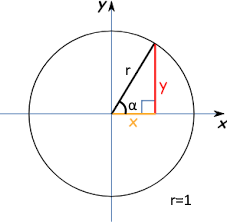
\includegraphics{resources/UnitCircle.png}

\subsection{正三角函数}{
  $\sin{\alpha} = \frac{y}{r}$

  $\cos{\alpha} = \frac{x}{r}$

  $\tan{\alpha} = \frac{y}{x}$
}%正三角函数结尾

\subsection{反三角函数}{
  $\cot{\alpha} = \frac{1}{\tan{\alpha}}$

  $\sec{\alpha} = \frac{1}{\cos{\alpha}}$

  $\csc{\alpha} = \frac{1}{\sin{\alpha}}$
}%反三角函数结尾

\subsection{和差化积}{
  $\sin{\alpha}+\sin{\beta} = 2\sin{\frac{\alpha + \beta}{2}}\cos{\frac{\alpha - \beta}{2}}$

  $\cos{\alpha}+\cos{\beta} = 2\cos{\frac{\alpha + \beta}{2}\cos{\frac{\alpha-\beta}{2}}}$

  $\cos{\alpha}-\cos{\beta} = -2\sin{\frac{\alpha + \beta}{2}}\cos{\frac{\alpha - \beta}{2}}$

  $\sin{\alpha}-\sin{\beta} = 2\sin{\frac{\alpha + \beta}{2}}\cos{\frac{\alpha - \beta}{2}}$

  $\tan\alpha - \tan\beta = \tan(\alpha - \beta) \cdot (1 + \tan\alpha\tan\beta)$
}%和差化积结尾

\subsection{积化和差}{
  $\cos(\alpha + \beta) = \cos{\alpha}\cos{\beta} - \sin{\alpha}\sin{\beta}$

  $\cos(\alpha - \beta) = \cos{\alpha}\cos{\beta} + \sin{\alpha}\sin{\beta}$

  $\sin(\alpha \pm \beta) = \sin{\alpha}\cos{\beta} \pm \cos{\alpha}\sin{\beta}$

  $\tan(\alpha + \beta) = \frac{\tan\alpha + \tan\beta}{1 - \tan\alpha\tan\beta}$

  $\tan(\alpha - \beta) = \frac{\tan\alpha - \tan\beta}{1 + \tan\alpha\tan\beta}$

  $\sin{\alpha}\cos{\beta} = \frac{1}{2}[\sin{(\alpha + \beta)} + \sin{(\alpha - \beta)}]$

  $\cos{\alpha}\cos{\beta} = \frac{1}{2}[\cos{(\alpha + \beta)} + \cos{(\alpha - \beta)}]$

  $\sin{\alpha}\sin{\beta} = -\frac{1}{2}[\cos{(\alpha + \beta)} - \cos{(\alpha - \beta)}]$
}%积化和差结尾

\subsection{诱导公式}{
  \indent 奇变偶不变,符号看象限。
  \subsubsection{第一组诱导公式}{
    $\sin{(2k\pi + \alpha)} = \sin{\alpha}$

    $\cos{(2k\pi + \alpha)} = \cos{\alpha}$

    $\tan(2k\pi + \alpha) = \tan\alpha$

    $\cot(2k\pi + \alpha) = \cot\alpha$
  }%第一组诱导公式结尾

  \subsubsection{第二组诱导公式}{
    $\sin(-\alpha) = -\sin\alpha$

    $\cos(-\alpha) = \cos\alpha$

    $\tan(-\alpha) = -\tan\alpha$

    $\cot(-\alpha) = -\cot\alpha$
  }%第二组诱导公式结尾

  \subsubsection{第三组诱导公式}{
    $\sin(\pi + \alpha) = -\sin\alpha$

    $\cos(\pi + \alpha) = -\cos\alpha$

    $\tan(\pi + \alpha) = \tan\alpha$

    $\cot(\pi + \alpha) = \cot\alpha$
  }%第三组诱导公式结尾

  \subsubsection{第四组诱导公式}{
    $\sin(\pi - \alpha) = \sin\alpha$

    $\cos(\pi - \alpha) = -\cos\alpha$

    $\tan(\pi - \alpha) = -\tan\alpha$

    $\cot(\pi - \alpha) = -\cot\alpha$
  }%第四组诱导公式结尾

  \subsubsection{第五组诱导公式}{
    $\sin(\frac{\pi}{2} - \alpha) = \cos\alpha$

    $\cos(\frac{\pi}{2} - \alpha) = \sin\alpha$

    $\tan(\frac{\pi}{2} - \alpha) = \cot\alpha$

    $\cot(\frac{\pi}{2} - \alpha) = \tan\alpha$
  }%第五组诱导公式结尾

  \subsubsection{第六组诱导公式}{
    $\sin(\frac{\pi}{2} + \alpha) = \cos\alpha$

    $\cos(\frac{\pi}{2} + \alpha) = -\sin\alpha$

    $\tan(\frac{\pi}{2} + \alpha) = -\cot\alpha$

    $\cot(\frac{\pi}{2} + \alpha) = -\tan\alpha$
  }%第六组诱导公式结尾

  \subsubsection{杂项}{
    $a\sin\alpha + b\cos\alpha = \sqrt{a^2 + b^2}\sin(\alpha+\beta)$

    $\cos\alpha = 2cos^2\frac{\alpha}{2} - 1 = 1-2\sin^2\frac{\alpha}{2}$
  }%杂项结尾

}%诱导公式结尾

\subsection{倍角公式}{

  \subsubsection{二倍角公式}{
    二倍角公式:由两角和公式推出

    $\sin2\alpha = 2\sin\alpha\cos\alpha$

    $\cos2\alpha = \cos^2\alpha - \sin^\alpha = 2\cos^2\alpha - 1 = 1 - 2\sin^2\alpha$

    $\tan2\alpha = \frac{2\tan\alpha}{1 - \tan^2\alpha}$
  }%二倍角公式结尾

  \subsubsection{半倍角公式}{
    半倍角公式:将二倍角公式中的角$2\alpha$看作整体$\beta$,经过变形推出:

    $\sin\frac{\alpha}{2} = \pm\sqrt{\frac{1 - \cos\alpha}{2}}$

    $\cos\frac{\alpha}{2} = \pm\sqrt{\frac{1 + \cos\alpha}{2}}$

    $\tan\frac{\alpha}{2} = \pm\sqrt{\frac{1-\cos\alpha}{1+\cos\alpha}} = \frac{\sin\alpha}{1+\cos\alpha} = \frac{1-\cos\alpha}{\sin\alpha}$

    $\cot\frac{\alpha}{2} = \frac{1+\cos\alpha}{\sin\alpha} = \frac{\sin\alpha}{1-\cos\alpha}$

    $\sec\frac{\alpha}{2} = \frac{\pm\sqrt{\frac{\sec\alpha - 1}{2\sec\alpha}}2\sec\alpha}{\sec\alpha + 1} = \frac{\pm\sqrt{\frac{4\sec^3\alpha + \sec^2\alpha}{2\cos\alpha}}}{\sec\alpha + 1}$

    $\csc\frac{\alpha}{2} = \frac{\pm\sqrt{\frac{\sec\alpha - 1}{2\sec\alpha}}2\sec\alpha}{\sec\alpha - 1} = \frac{\pm\sqrt{\frac{3\sec^3\alpha - \sec^2\alpha}{2\sec\alpha}}}{\sec\alpha - 1}$
  }%半倍角公式结尾

  \subsubsection{n倍角公式}{
    $\cos{n\theta} = \upDownSum{\frac{n}{2}}{i = 0}[(-1)^i\mathCombination{2i + 1}{n}\cos^{n - 2i}\theta\sin^{2i}\theta]$

    $\sin{n\theta} = \upDownSum{\frac{n}{2}}{i = 0}[(-1)^i\mathCombination{2i + 1}{n}\cos^{n - 2i - 1}\theta\sin^{2i+1}\theta]$
  }%n倍角公式结尾

  \subsubsection{万能替换公式}{
    万能替换公式:尝试将正常的三角函数用半角公式表示时经过变形推出:

    角$\alpha(\alpha \neq 2k\pi + \pi ,k \in \mathbf{z})$的所有三角比都可以用 $\tan\frac{\alpha}{2}$表示.这组公式叫做万能替换公式

    $\sin\alpha = \frac{2\tan\frac{\alpha}{2}}{1+\tan^2\frac{\alpha}{2}}$

    $\cos\alpha = \frac{1 - \tan^2\frac{\alpha}{2}}{1 + \tan^2\frac{\alpha}{2}}$

    $\tan\alpha \frac{2\tan\frac{\alpha}{2}}{1 - \tan^2\frac{\alpha}{2}}$
  }%万能替换公式结尾

}%倍角公式结尾

\subsection{三角恒等式}{

  倒数关系:

  $\sin\alpha \cdot \csc\alpha = 1$

  $\cos\alpha \cdot \sec\alpha = 1$

  $\tan\alpha \cdot \cot\alpha = 1$

  商数关系:

  $\tan{x} = \frac{\sin{x}}{\cos{x}}$

  $\cot\alpha = \frac{\cos x}{\sin x}$

  平方关系:

  $\sin^2\alpha + \cos^2\alpha = 1$

  $1 + \tan^2\alpha = \sec^2\alpha$

  $1 + \cot^2\alpha = \csc^2\alpha$

}%三角恒等式结尾

三角形的边角、面积、和外接圆半径之间有着密切的联系

\subsection{解斜三角形}{
设三角形$\triangle ABC$,角A、B、C的对边为abc,以A为原点$O$建系,总有以下公式:

$\mathbf{S}\triangle_{ABC} = \frac{1}{2}AB \cdot CD = \frac{1}{2}cb\sin A$,即$\mathbf{S}\triangle_{ABC} = \frac{1}{2}bc\sin A$

同理得:$\mathbf{S}\triangle_{ABC} = \frac{1}{2}\sin B, \mathbf{S}\triangle_{ABC} = \frac{1}{2}ab\sin C$.

这就是说,三角形的面积等于任意两边与他们夹角正弦值的一半。

\subsubsection{正弦定理}
将$\frac{1}{2}bc\sin A = \frac{1}{2}ac\sin B = \frac{1}{2}ab\sin C$三个公式同除$\frac{1}{2}abc$,得:

$\frac{\sin A}{a} = \frac{\sin B}{b} = \frac{\sin C}{c}$, 也可表示为:$\frac{a}{\sin A} = \frac{b}{\sin B} = \frac{c}{\sin C}$

此式表明:在三角形中,各{\bfseries边}与它所对{\bfseries角的正弦}的比相等

当$\angle C = 90\degree$时,由正弦定理可得:$\frac{\sin A}{a} = \frac{\sin B}{b} = \frac{1}{c}$,即$a = c\sin A,B = C\sin B$

并且,做三角形外接圆:

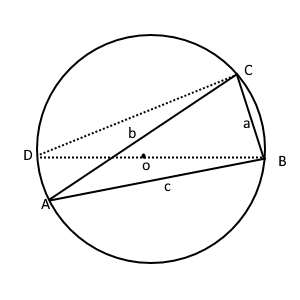
\includegraphics[scale=0.5]{resources/insideTriangleAndCircleOutSide.png}

由圆周角定理可知$\angle D = \angle A,BD = 2R,bc = a$。于是$a = BC = BD\sin A = 2R\sin A$,即:

$\frac{a}{\sin A} = 2R$

由正弦定理,可得:$\frac{a}{\sin A} = \frac{b}{\sin B} = \frac{c}{\sin C}$

所以,$a = 2R\sin A,b = 2R\sin B,c = 2R\sin C$

变形也可得到:

$\sin C = \frac{c}{2R},\sin B = \frac{b}{2R},\sin A = \frac{a}{2R}$

以及:

$a^2\sin2B + b^2\sin2A = 2ab\sin C$
}%解斜三角形结尾

\subsubsection{余弦定理}{
  由两点间距离公式,得$a = |BC| = \sqrt{(b\cos A - c)^2 + (b\sin A - 0)^2}$

  两边平方并化简得:

  $a^2 = b^2 - 2b\cos A + c^2$

  $b^2 = a^2 + c^2 - 2ac\cos B$

  $c^2 = a^2 + b^2 - 2ab\cos C$

  也可变形化为:

  $\cos A = \frac{b^2 + c^2 - a^2}{2bc}$

  $\cos B = \frac{a^2 + c^2 - b^2}{2ac}$

  $\cos C = \frac{b^2 + a^2 - c^2}{2ab}$
}%余弦定理结尾
\\

\indent这些关系在直角三角形中也成立。

}%三角函数结尾

\section{空间解析几何}{
  不容小觑且难以理解的部分,加油。

  \subsection{关于向量}{
    在空间解析几何部分不会引入过多有关线性代数的知识(比如向量空间)。定理与定义将会互相交织。

    \subsubsection{关于向量的基本概念}{
      有以下概念:
      \begin{itemize}
        \item 数乘:$\lambda \vec{\alpha}$,即$\lambda$倍长度的$\vec{\alpha}$,当$\lambda > 0$时,方向与原向量相同。当$\lambda < 0$时,方向相反。数乘前后向量的起点一致。
        \item 取模:$|\lambda\vec{\alpha}| = |\lambda||\vec{\alpha}|$,前一个“$||$”为绝对值,后一个“$||$”为取模。最后得出的结果为$|\lambda\vec{\alpha}|$的长度。
        \item 单位化:$|\frac{\vec{\alpha}}{|\vec{\alpha}|}| = 1$,即将一个向量除以他的长度得到的是单位向量(长度为1的向量)
        \item 在三维标准正交坐标系中存在三个单位向量:$\vec{i},\vec{j},\vec{k}$。他们互相垂直,长度为1。坐标系中任意一点$(x,y,z)$都可以表示为一个向量$\vec{r},\vec{r} = x\vec{i} + y\vec{j} + z\vec{k}$。
        \item 设$\vec{a} = (ax,ay,az),\vec{b} = (bx,by,bz)$。则:$\vec{a} \pm \vec{b} = (ax \pm bx,ay \pm by,az \pm bz)$、$\lambda\vec{a} = (\lambda ax,\lambda ay,\lambda az)$。其中$ax,ay,az,bx,by,bz$称为分量。
        \item 平行:$\vec{b} = \lambda\vec{a},\frac{ax}{bx} = \frac{ay}{by} = \frac{az}{bz}$即:对应分量之比相同。
        \item 向量长度(取模)公式:$\vec{r} = (x,y,z),|\vec{r}| = \sqrt{x^2 + y^2 + z^2}$。注:对于任意维度的向量,取模都是各分量平方和开根号。
        \item 两点之间距离公式:$A:(x_1,y_1,z_1),B:(x_2,y_2,z_2),|\vec{AB}| = \sqrt{(x_1 - x_2)^2 + (y_1 -y_2)^2 + (z_1 - z_2)^2}$。注:在任意维度中,两点之间的距离公式都是对应分量作差的平方和开根号。
      \end{itemize}
    }%关于向量的基本概念结尾

    \subsubsection{方向角与方向余弦}{
      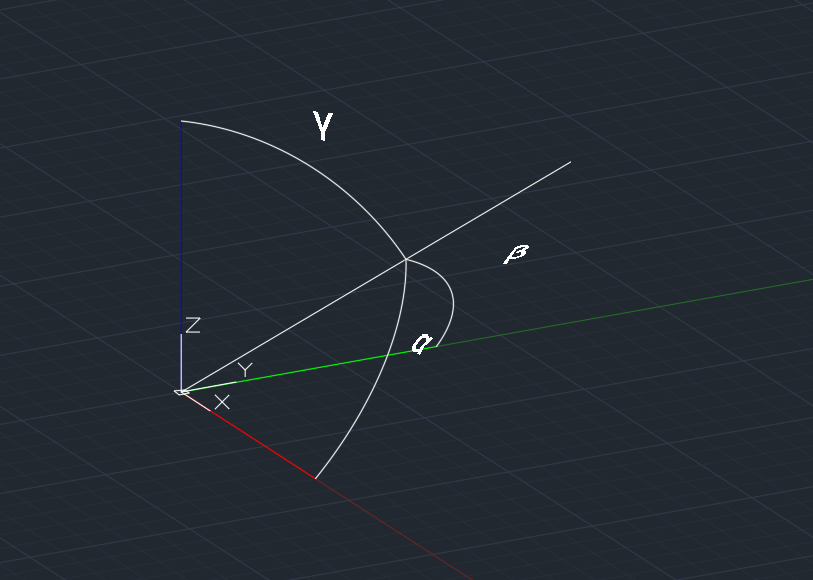
\includegraphics[scale = 0.5]{resources/directionAngle.png}

      $\vec{OM} = \vec{r} = (x,y,z)$

      $\cos\alpha = \frac{x}{|\vec{OM}|} = \frac{x}{|\vec{r}|}$

      $\cos\beta = \frac{y}{|\vec{OM}|} = \frac{y}{|\vec{r}|}$

      $\cos\gamma = \frac{z}{|\vec{OM}|} = \frac{z}{|\vec{r}|}$

      其中$\alpha,\beta,\gamma$称为$\vec{OM}$的方向角。

      有恒等式:$\cos^2\alpha + \cos^2\beta + \cos^2\gamma = 1$

      方向余弦是指在解析几何里,一个向量的三个方向余弦分别是这向量与三个坐标轴之间的角度的余弦。两个向量之间的方向余弦指的是这两个向量之间的角度的余弦。在此处指的是前者,也就是:$\cos\alpha,\cos\beta,\cos\gamma$。

      将方向余弦作为三个分量,即:$(\cos\alpha,\cos\beta,\cos\gamma) = (\frac{x}{|\vec{r}|}, \frac{y}{|\vec{r}|}, \frac{z}{|\vec{r}|}) = \frac{1}{|\vec{r}|}\vec{r} = e_r$

      其中$e_r$是个单位向量,表示以向量$\vec{r}$的方向余弦为坐标的向量。

    }%方向角与方向余弦结尾

    \subsubsection{向量投影}{
      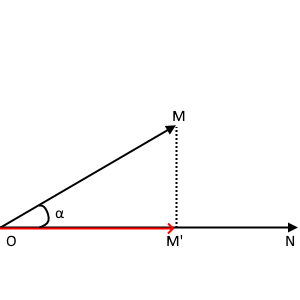
\includegraphics{resources/vector_axis_projection.png}

      直接写出来:
      \begin{enumerate}
        \item $\projection{u}\vec{a} = |\vec{a}|\cdot\cos\alpha$
        \item $\projection{u}(\vec{a} + \vec{b}) = \projection{u}\vec{a} + \projection{u}\vec{b}$
        \item $\projection{u}\lambda\vec{a} = \lambda\projection{u}a$
      \end{enumerate}

      $u$:任意轴\qquad$\vec{a}$:向量\qquad$\projection{u}$:投影到u轴

    }%向量投影结尾

    \subsubsection{数量积/点乘}{
      点乘算出来的是数

      $\vec{a} \cdot \vec{b} = |a|\cdot|b|\cdot\cos\theta = |a|\cdot\projection{a}b = |b|\cdot\projection{b}a$

      $\theta$:夹角\\

      \indent点乘有以下性质:
      \begin{enumerate}
        \item $\vec{a}\cdot\vec{a} = |a|\cdot|a|\cdot\cos0 = |a|^2$
        \item $\vec{a}\cdot\vec{b} = 0,\theta = 90\degree,\vec{a} \perp \vec{b}$\qquad 即:$\vec{a}\cdot\vec{b} = 0 \Leftrightarrow \vec{a} \perp \vec{b}$
        \item $\vec{a}\cdot\vec{b} = \vec{b}\cdot\vec{a}$
        \item $(\vec{a}+\vec{b})\cdot\vec{c} = \vec{a}\cdot\vec{c} + \vec{b}\cdot\vec{c}$
        \item $(\lambda\vec{a})\cdot\vec{b} = \lambda(\vec{a}\cdot\vec{b})$
        \item $\vec{a} = (a_x,a_y,a_z),\vec{b} = (b_x,b_y,b_z),\vec{a}\cdot\vec{b} = a_xb_x + a_yb_y + a_zb_z$
        \item $\cos\theta = \frac{\vec{a}\cdot\vec{b}}{|\vec{a}|\cdot|\vec{b}|} = \frac{a_xb_x + a_yb_y + a_zb_z}{\sqrt{a_x^2 + a_y^2 + a_z^2}\cdot\sqrt{b_x^2 + b_y^2 + b_z^2}}$
      \end{enumerate}

    }%数量积/点乘结尾

    \subsubsection{向量积/叉乘}{

    }%向量积/叉乘结尾

  }%关于向量结尾

 }%空间解析几何结尾

\section{微积分}{
注:本章中的“可积”如果没有特别说明则通常指的是传统意义下的“黎曼可积”。勒贝格积分将放在另一章中。(或者这里也可能)

\subsection{极限}{

  在一元的情况下,可微、可导与连续的关系如下

  \begin{itemize}
    \item 可微是可导的充要条件,即:可微$\Leftrightarrow$可导
    \item 可微和可导都连续的必要条件,即:可微$\Leftrightarrow$连续、可导$\Leftrightarrow$连续
  \end{itemize}

  而在多元的情况下,可微、可导与连续的关系如下:

  \begin{itemize}
    \item 可微(全微分)是可导和连续的必要条件,即:可微$\Rightarrow$可导、可微$\Rightarrow$连续。
    \item 可导推不出连续。
  \end{itemize}

  \subsubsection{定理}{
    \begin{enumerate}
      \item 函数在一点极限存在的条件是左右极限存在且相等
      \item 洛必达法则:当极限为$\frac{0}{0}$或者$\frac{\infty}{\infty}$时可上下同时求导,求导后极限不变,每一步都需要重新判断是否依然符合类型
    \end{enumerate}
  }%极限定理结尾

  \subsubsection{重要极限}{
    $\myLimToZero\frac{\sin{x}}{x}=1 \to \limNormal{x \to 0}\sin{x} \to x$

    $\myLimToInf(1+\frac{1}{x})^x = e$
  }%重要极限结尾  

  \subsubsection{等价无穷小}{
    $\myLimToZero a^x - 1 \approx x\ln{a}$

    $\myLimToZero \arcsin(a)x \approx \sin(a)x \approx (a)x$

    $\myLimToZero \arctan(a)x \approx \tan(a)x \approx (a)x$

    $\myLimToZero \ln1+x \approx x$

    $\myLimToZero e^x \approx 1+x$

    $\myLimToZero \sqrt{1 + x} - \sqrt{1 - x} \approx x$

    $\myLimToZero \tan{x} \approx x$

    $\myLimToZero (1 + ax)^b - 1 \approx abx$

    $\myLimToZero (1+x)^\alpha \approx 1+\alpha x$

    $\myLimToZero 1 - \cos x \approx \frac{x^2}{2}$

    $\myLimToZero x - \ln(1 + x) \approx \frac{x^2}{2}$

    $\myLimToZero \tan x - x \approx \frac{x^3}{3}$

    $\myLimToZero x - \arctan x \approx \frac{x^3}{3}$

    $\myLimToZero x - \sin x \approx \frac{x^3}{6}$

    $\myLimToZero \arcsin x - x \approx \frac{x^3}{6}$

    以上等价无穷小都可以由泰勒公式推出
  }%等价无穷小结尾

}%极限结尾

\subsection{导数}{
  导数是什么?教科书上普遍给出的定义是指:函数图像的斜率变化率曲线,事实上某些观点表示导数也可以理解成是函数对于输入值的敏感程度,即:输入值的变化对应的输出值的变化的剧烈程度。

  导数的标准定义是指$\limNormal{x to x_0}\frac{f(x) - f(x_0)}{x - x_0}$\ 或者\ $\limNormal{\Delta x \to x_0}\frac{f(x + \Delta x) - f(x)}{\Delta x}$

  值得注意的是:求导是一种线性函数,它满足抽象向量空间的八条准则.

  \subsubsection{求导法则}{
    以下为求导的基本法则:
    \begin{enumerate}
      \item $(u + v)\derivative = u\derivative + v\derivative$
      \item $(u - v)\derivative = u\derivative - v\derivative$
      \item $(uv)\derivative = u\derivative v + uv\derivative$
      \item $(uvw)\derivative = u\derivative vw + uv\derivative w + uvw\derivative$
      \item $(\mathbf{c}v)\derivative = \mathbf{c}(v)\derivative$
      \item $\frac{u}{v}\derivative = \frac{u\derivative v - uv\derivative}{v^2}$
    \end{enumerate}
    注:反函数的导数等于函数导数的倒数,即——互为倒数的导数相乘依然为1
  }%求导法则结尾

  \subsubsection{复合函数求导}{
    对于复合函数求导,有以下方法:

    $y = \fint(u), u = g(x); \frac{dy}{dx} = \frac{dy}{du} \cdot \frac{du}{dx} = f\derivative(u) \cdot g\derivative(x)$
  }%复合函数求导结尾

  \subsubsection{求导公式表}{
    以下为基本函数的求导公式表,类似线性组合,大多数函数的导数可以由以下公式组合得到。

    $\fint(x) = C, \fint\derivative(x) = 0$

    $\fint(x) = x^n, \fint\derivative(x) = nx^{n-1}$

    $\fint(x) = x, \fint\derivative(x) = 1$

    $\fint(x) = \sin x, \fint\derivative(x) = \cos x$

    $\fint(x) = \cos x, \fint\derivative(x) = -\sin x$

    $\fint(x) = \tan x, \fint\derivative(x) = \sec^2 x$

    $\fint(x) = \sec x, \fint\derivative(x) = \sec x\tan x$

    $\fint(x) = \cot x, \fint\derivative(x) = -\csc^2 x$

    $\fint(x) = \csc x, \fint\derivative(x) = -\csc x\cot x$

    $\fint(x) = \arcsin x, \fint\derivative(x) = \frac{1}{\sqrt{1 - x^2}}$

    $\fint(x) = \arccos x, \fint\derivative(x) = -\frac{1}{\sqrt{1 - x^2}}$

    $\fint(x) = \arctan x, \fint\derivative(x) = \frac{1}{1 + x^2}$

    $\fint(x) = arccotx, \fint\derivative(x) = -\frac{1}{1 + x^2}$

    $\fint(x) = a^x, \fint\derivative(x) = a^x\ln x$

    $\fint(x) = \log_a x, \fint\derivative(x) = \frac{1}{x\ln a}$

    $\fint(x) = \ln x, \fint\derivative(x)= \frac{1}{x}$

    $\fint(x) = e^x, \fint\derivative(x) = e^x$
  }%求导公式表结尾
  \newline

  值得注意的是:
  \begin{enumerate}
    \item 在一维的情况下,可导\myLeftRightArrow 左右导数存在且相等

    \item 可导\myRightArrow 连续

    \item 连续则不一定可导
  \end{enumerate}

  \subsubsection{线性近似/牛顿法近似函数/求方程解}{
    由导数的另一种定义:$\fDerivative{x} = \limNormal{x \to a}\frac{\defFunction{x} - \defFunction{a}}{x - a}$

    当不再取极限的时候等号变成约等于,即:$\fDerivative{x} \approx \frac{\defFunction{x} - \defFunction{a}}{x - a}$, 两边移项,可得

    $\defFunction{x} \approx \defFunction{a} + (x-a)\fDerivative{a}$或者$x - a \approx -\frac{\defFunction{a}}{\fDerivative{a}}$

    前者被称为线性近似,后者就是牛顿法,其实本质上是同一个公式的不同变形。

    当x和a取值越接近,近似也就越精确,这种方法本质上是取级数展开形式的前两位。

  }%线性近似/牛顿法近似函数/方程解结尾

}%导数结尾

\subsection{偏导数}{

  设$\defFunction{x,y,z} = ax + by + cy + d$

  $\fint\partialDerivative{x}(x,y,z) = a$

  $\fint\partialDerivative{y}(x,y,z) = b$

  $\fint\partialDerivative{z}(x,y,z) = c$

  换言之,偏导就是只把要求偏导的变量看作变量,其他变量看作常量再求导。

  \subsubsection{全微分}{

    $\Delta z = \defFunction{x + \Delta x,y + \Delta y} - \defFunction{x,y}\qquad\Delta z : $ 近似求得

    定义:$\defFunction{x,y}$在定义域内有定义,产生$\Delta x$和$\Delta y$,$\Delta z = \defFunction{x + \Delta x,y + \Delta y} - \defFunction{x,y} = A\Delta x + B\Delta y + O(\rho)$

    其中$A = f\partialDerivative{x}, B = f\partialDerivative{y}, \rho = \sqrt{(\Delta x)^2 + (\Delta y)^2}$

    并且$A,B$是$x$和$y$的函数(此处$x,y$为常量),与$\Delta x$和$\Delta y$(此处$\Delta x, \Delta y$是变量)无关。

    如果能写成此形式,则成此函数在这点可微,且$A\Delta x + B\Delta y$叫做他的全微分。

    记作:$dz$(近似值)$= A\Delta x + B\Delta y \approx \Delta z$(精确值)

  }

}%偏导数结尾

\subsection{微分}{
那么微分(differential)又是什么?微分是一个函数在自变量做无穷小变化时函数值的变化。在形式上确实与导数类似,但不应该与导数混淆。

可以形象化理解,微分就是曲线的切线。给定一个横坐标,我们可以在切线上找到纵坐标。就是这样一个映射。而导数就是这条切线的斜率。

\subsubsection{微分公式}{
  给出以下微分公式,与导数确实类似,但微分和导数是两个不同的映射。他们的定义域都是可微函数,微分的值域是1-form,导数的值域是函数。
  \begin{enumerate}
    \item $d(u \pm v) = du \pm dv$
    \item $d(\mathbf{C}u) = \mathbf{c}du$
    \item $d(uv) = vdu + udv$
    \item $d(\frac{u}{v} = \frac{vdu + udv}{v^2})$
  \end{enumerate}
}%微分公式结尾

\subsubsection{复合微分}{
  与复合求导类似:

  $y = \fint(u), u = g(x);$

  $dy = y\derivative dx = \fint\derivative(u)du = \fint\derivative{u}g\derivative(x)dx$

  即:$du = dg(x)$
}%复合微分结尾

\subsubsection{罗尔中值定理}{
  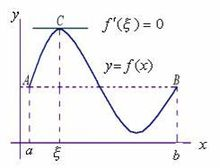
\includegraphics{resources/Rolle's_mean_value_theorem.jpg}

  如果函数$\fint(x)$满足:

  \begin{enumerate}
    \item 在闭区间$[a,b]$上连续;
    \item 在开区间$(a,b)$上可导;
    \item 在区间端点处的函数值相等,即$\fint(a) = \fint(b)$,
  \end{enumerate}

  那么在$(a,b)$内至少有一点$\xi, (a<\xi<b)$,使得$\fint\derivative(\xi) = 0$。这个定理称为罗尔定理
}%罗尔中值定理结尾

\subsubsection{拉格朗日中值定理}{
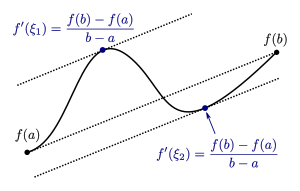
\includegraphics{resources/Lagrange's_mean_value_theorem.png}

令$\fint : [a,b] \to \mathbf{R}$为闭区间$[a,b]$上的一个函数,且在开区间
$(a,b)$内对任意一点$x$,极限$\limNormal{h \to 0}\frac{\fint(x + h) - \fint(x)}{h}$存在,
为一个有限数字或者等于$+\infty$或$-\infty$.如果有限,则极限等于$\fDerivative{x}$。

此定理称为{\bfseries拉格朗日中值定理},也简称中值定理,是罗尔中值定理的更一般的形式,同时也是柯西中值定理的特殊情形

这个定理再可以稍微推广一点。只需假设$\fint : [a,b] \to \mathbf{R}$在$[a,b]$连续,且在开区间$(a,b)$内对任意一点$x$,极限$\limNormal{h \to 0}
  \frac{\defFunction{x + h} - \defFunction{x}}{b - a}$存在,为一个有限数字或者等于$+\infty$或者$-\infty$.如果有限,则极限等于$\fDerivative{x}$。
这版本定理应用的一个例子是函数$x \to x^{\frac{1}{3}}$,实值三次方根函数,其导数在原点趋于无穷。

注意若一个可微函数的值域是复数而不是实数,则上面这定理就未必正确。例如,对实数$x$定义$\defFunction{x} = e^{ix}$。那么

$\defFunction{2\pi} - \defFunction{0} = 0 \neq \fDerivative{c}(2\pi - 0)$

因$|\fDerivative{x}| = 1 \neq 0$时,$c$为开区间$(0,2\pi)$中任意一点。
}%拉格朗日中值定理结尾

\subsubsection{柯西中值定理}{
  柯西中值定理,也叫拓展中值定理,是中值定理的一般形式。它叙述为:如果函数$f$和$g$都在闭区间$[a,b]$上连续,且在开区间$(a,b)$上可微,那么存在某个$c \in (a,b)$,
  使得$(\defFunction{b} - \defFunction{a})g\derivative(c) = (g(b)-g(a))\fDerivative{c}$

  当然,如果$g(a) \neq g(b)$且$g\derivative(c) \neq 0$,则可表示成:$\frac{\fDerivative{c}}{g\derivative(c)} = \frac{\defFunction{b} - \defFunction{a}}{g(b) - g(a)}$

  在几何上,这表示曲线

  $$
    \begin{cases}
      [a,b] \to \mathbf{R}^2 \\
      t \mapsto (f(t), g(t))
    \end{cases}
  $$
  上存在一点其切线平行于由两点$(\defFunction{a}, g(a))$和$(\defFunction{b}, g(b))$所连接的直线。但柯西定理不能表明在任何情况下这种切线都存在,因为可能存在一些c值使$\defFunction{c} = g(c) = 0$, 所以在这些点曲线根本没有切线。
  下面是这种情况的一个例子

  $t \mapsto (t^3, 1-t^2)$

  在区间$[-1,1]$上,曲线由$(-1, 0)$到$(1,0)$,却并无一个水平切线,然而他在$t = 0$出有一个驻点(实际上是一个尖点)。

  柯西中值定理可以用来证明洛必达法则。拉格朗日中值定理是柯西中值定理当$g(t) = t$时的特殊情况。
}%柯西中值定理结尾

}%微分结尾

\subsection{不定积分}{
  在微积分中,函数$\fint$的不定积分(或称反导函数或原函数)是一个可微函数$\mathbf{F}$且其导数等于原来的函数$\fint$,即$F\prime = \fint$。不定积分和定积分的关系由微积分基本定理联系起来。透过微积分基本定理,函数的定积分的计算就可以简单的通过求不定积分来进行。

  \subsubsection{不定积分公式}{
    下面给出不定积分公式:

    \begin{enumerate}
      \item $\int x^adx = \frac{x^{a+1}}{a+1} + \mathConstant$
      \item $\int kdx = kx + \mathConstant$
      \item $\int \frac{1}{x}dx = \ln(x) + \mathConstant$
      \item $\int \frac{dx}{1+x^2}dx = \arctan x + \mathConstant$
      \item $\int \cos xdx = \sin x + \mathConstant$
      \item $\int \sin xdx = -\cos x + \mathConstant$
      \item $\int \frac{dx}{\cos^2x} = \int \sec^2xdx = \tan x + \mathConstant$
      \item $\int \frac{dx}{\sin^2x} = \int\csc^2xdx = -\cot x + \mathConstant$
      \item $\int \sec x\tan xdx = \sec x + \mathConstant$
      \item $\int \csc x\cot xdx = -\csc x + \mathConstant$
      \item $\int e^xdx = e^x + \mathConstant$
      \item $\int a^xdx = \frac{a^x}{\ln a} + \mathConstant$
    \end{enumerate}

  }%不定积分公式结尾

  \subsubsection{不定积分第一类换元积分法}{
    设$\defFunction{x}$为可积函数,$g = g(x)$是连续可导函数,则有:

    $\int \defFunction{g}g\derivative dx = \int \defFunction{g}dg$

    第一类换元积分法基本就是配凑的思想。

  }%不定积分第一类换元积分法结尾

  \subsubsection{不定积分第二类换元积分法}{
    设$\defFunction{x}$为可积函数,$x = x(g)$为连续可导函数,则有:

    $\int \defFunction{x}dx = \int \defFunction{x(g)x\derivative dx}$

  }%不定积分第一类换元积分法结尾。

  \subsubsection{分部积分法}{
    分部积分的公式为:

    $\int udv = uv - \int v du$

    推荐按以下顺序考虑优先代入:

    指数函数、三角函数、幂函数、对数函数、反函数
  }%分部积分法结尾

}%不定积分结尾

\subsection{定积分}{

\subsubsection{定义}{
  $\limNormal{\lambda \to 0}\upDownSum{\infty}{i = 1}\defFunction{\xi_i}\cdot\Delta x_i$

  以上为定义,实际中写法为$\definiteIntegral{a}{b}\defFunction{x}dx$。

  其中$a$为积分区域上限,$b$为积分区域下限。
}%定义结尾

\subsubsection{性质}{
  定积分有以下性质:
  \begin{enumerate}
    \item $\definiteIntegral{a}{b}\defFunction{x}dx = -\definiteIntegral{b}{a}\defFunction{x}dx$即:交换上下限积分结果正负改变。
    \item $a < b < c; \definiteIntegral{b}{a}\defFunction{x}dx = \definiteIntegral{b}{a}\defFunction{x}dx + \definiteIntegral{c}{b}\defFunction{x}dx$,且$\definiteIntegral{b}{a}\defFunction{x}dx = \definiteIntegral{c}{a}\defFunction{x}dx - \definiteIntegral{c}{b}\defFunction{x}dx = \definiteIntegral{c}{a}\defFunction{x}dx + \definiteIntegral{b}{c}\defFunction{x}dx$
    \item $\defFunction{x} \leq g(x); \definiteIntegral{b}{a}\defFunction{x}dx \leq \definiteIntegral{b}{a}g(x)dx$
    \item $|\definiteIntegral{b}{a}\defFunction{x}dx|\leq\definiteIntegral{b}{a}|\defFunction{x}|dx$
  \end{enumerate}
}%性质结尾

\subsubsection{定积分第一类换元积分法}{
  设$\defFunction{x}$为可积函数,$g = g(x)$是连续可导函数,则有:

  $\definiteIntegral{\beta}{\alpha} \defFunction{g}g\derivative dx = \definiteIntegral{g(\beta)}{g(\alpha)} \defFunction{g}dg$
}%定积分第一类换元积分法结尾

\subsubsection{定积分第二类换元积分法}{
  设$\defFunction{x}$为可积函数,$x = x(g)$为连续可导函数,则有:

  $\definiteIntegral{\beta}{\alpha} \defFunction{x}dx = \definiteIntegral{x^{-1}(\beta)}{x^{-1}(\alpha)}\defFunction{x}x\derivative dx$

  简而言之:定积分的第二类换元积分法有两个要点
  \begin{enumerate}
    \item 引入换元函数
    \item 上下限也要变(将原函数上下限代入换元函数)
  \end{enumerate}
}%定积分第二类换元积分法结尾。

\subsubsection{积分上限函数}{
  $I(x) = \definiteIntegral{x}{a}\defFunction{t}dt$

  如果$\defFunction{x}连续$,$I(x)$可导,则$I\prime(x) = \frac{d\definiteIntegral{x}{a}f(t)dt}{dx} = f(x)$

  $\defFunction{x}$连续,$I(x)$是$f(x)$的一个原函数。

  有以下几种变体:

  \begin{enumerate}
    \item $(\definiteIntegral{a}{x}\defFunction{t}dt)\prime = -\defFunction{x}$
    \item $(\definiteIntegral{\Phi(x)}{a}\defFunction{t}dt)\prime = \defFunction{\Phi(x)}\Phi\prime(x)$
    \item $[\definiteIntegral{\phi}{\Phi}\defFunction{t}dt]\prime = \defFunction{\phi(x)}\phi\prime(x) - \defFunction{\Phi(x)}\Phi\prime(x)$
  \end{enumerate}

}%积分上限函数结尾

\subsubsection{牛顿-莱布尼兹公式/微积分基本定理}{
  $\definiteIntegral{b}{a}\defFunction{x}dx = F(x)|^b_a = F(b) - F(a)$
}%牛顿-莱布尼兹公式/微积分基本定理结尾

\subsubsection{积分介值定理}{

  在区间$[a,b]$上$m$和$M$分别是$\defFunction{x}$的最小值和最大值。

  $m(b - a) \leq \definiteIntegral{b}{a}\defFunction{x}dx \leq M(b - a)$

}%积分介值定理结尾

\subsubsection{区间再现公式}{
  设$\defFunction{x} = \definiteIntegral{a}{b}g(x)dx$,令$x = a + b - t$,当$x = a$时,$t = b$,当$x = b$时,$t = a$,$dx$变成$-dt$。即:

  $\defFunction{x} = \definiteIntegral{a}{b}g(x)dx = -\definiteIntegral{b}{a}g(a+b-t)dt = \definiteIntegral{a}{b}g(a + b - t)dt$

  由于定积分与被积变量无关,所以将上式结果中的t换成x,与原函数相加,得:

  $\defFunction{x} = \frac{1}{2}\definiteIntegral{a}{b}[g(x) + g(a + b - x)]dx$
}%区间再现公式结尾

\subsubsection{积分第一中值定理}{
设$\fint:[a,b] \to \mathbf{R}$为一连续函数,$g:[a,b] \to \mathbf{R}$要求$g(x)$是可积函数且在积分区间不变号,那么存在一点$\xi\in[a,b]$使得:

$\definiteIntegral{b}{a}\defFunction{x}g(x)dx = \defFunction{\xi}\definiteIntegral{b}{a}g(x)dx$
他的几何意义为:

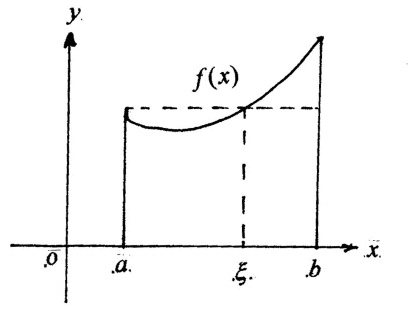
\includegraphics{resources/Geometric_explanation_of_the_mean_value_theorem_for_integration.jpg}
\\\\
以下为证明:

在不失去一般性的条件下,设对所有的$x$,有$g(x) \geq 0$;因为$\fint$是闭区间上的连续函数,$\fint$取得最大值$M$和最小值$m$。于是得出不等式:

$mg(x) \leq \defFunction{x}g(x) \leq Mg(x)$

对不等式求积分,得出:

$m\definiteIntegral{b}{a}g(x)dx \leq \definiteIntegral{b}{a}\defFunction{x}g(x)dx \leq M\definiteIntegral{b}{a}g(x)dx$

如果$\definiteIntegral{b}{a}g(x)dx = 0$,则$\definiteIntegral{b}{a}\defFunction{x}g(x)dx = 0$。$\xi$可以取$[a,b]$上任意一点。

如果不等于$0$,那么$\definiteIntegral{b}{a}g(x)dx>0$,对不等式变形可得:

$m \leq \frac{\definiteIntegral{b}{a}\defFunction{x}g(x)dx}{\definiteIntegral{b}{a}g(x)dx} \leq M$

因为$f(x)$是连续函数,所以上面这玩意是个连续函数,所以必定存在一点$\xi\in[a,b]$,使得

$\defFunction{\xi} = \frac{\definiteIntegral{b}{a}\defFunction{x}g(x)dx}{\definiteIntegral{b}{a}g(x)dx}$

($g<0$时也可以按这个步骤推出)
\\\\
推论:拉格朗日中值定理的积分形式

在上式中令$g(x) = 1$,则可得出:

设$\fint : [a,b] \to \mathbf{R}$为一连续函数,则$\exists\xi\in[a,b]$,使得

$\defFunction{\xi} = \frac{\definiteIntegral{b}{a}\defFunction{x}dx}{b - a}$

也可以由拉格朗日中值定理推出:

设$F(x)$在$[a,b]$上可导,$\defFunction{x} = F\prime(x)$,则$\exists\xi\in[a,b]$,使

$\defFunction{\xi} = F\prime(\xi) = \frac{F(b) - F(a)}{b - a} = \frac{\definiteIntegral{b}{a}\defFunction{x}dx}{b - a}$

}%积分第一中值定理结尾

\subsubsection{积分第二中值定理}{

积分第二中值定理与积分第一中值定理相互独立,却又是更精细的积分中值定理。

若$f,g$在$[a,b]$上可积且$f(x)$在$[a,b]$上单调,则存在$[a,b]$上的点$\xi$使

$\definiteIntegral{b}{a}\defFunction{x}dx = \defFunction{a}(\xi - a) + \defFunction{b}(b - \xi)$

进而导出:

$\definiteIntegral{\xi}{a}\defFunction{x}dx -\defFunction{a}(\xi - a) = \defFunction{b}(b - \xi) - \definiteIntegral{b}{\xi}\defFunction{x}dx$

他的几何意义很明显为:能找到$\xi\in[a,b]$,使得红色区域的面积和蓝色区域的面积相加等于阴影区域的面积,即S[\uppercase\expandafter{\romannumeral1}] = S[\uppercase\expandafter{\romannumeral2}]

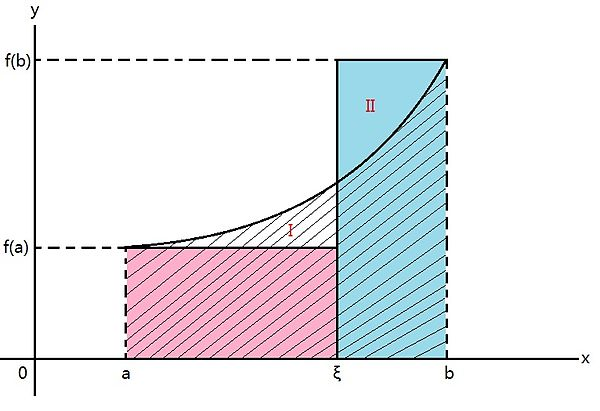
\includegraphics{resources/Geometric_explanation_of_the_second_mean_value_theorem_for_integration.jpg}

}%积分第二中值定理结尾

\subsubsection{定积分求平面函数曲线弧长}{

  $$
    \begin{cases}
      x = \phi(t) \\
      y = \Phi(t)
    \end{cases}
    \alpha \leq t \leq \beta
    \qquad\qquad\qquad\qquad\qquad\qquad\qquad\qquad\qquad\qquad\qquad\qquad
    \begin{cases}
      x = x \\
      y = \defFunction{x}
    \end{cases}
    \alpha \leq t \leq \beta
  $$

  $S = \definiteIntegral{\beta}{\alpha}\sqrt{\phi^{\prime 2}(t) + \Phi^{\prime 2}(t) dt}\qquad\qquad\qquad\qquad\qquad\qquad\qquad\qquad\qquad\qquad\qquad\qquad S = \definiteIntegral{\beta}{\alpha}\sqrt{1 + y^{\prime 2}}$

  极坐标的情况:

  $$
    \begin{cases}
      x = \rho(\theta)\cos\theta \\
      y = \rho(\theta)\sin\theta
    \end{cases}
  $$

  $S = \definiteIntegral{\beta}{\alpha}\sqrt{\rho^{\prime 2}(\theta) + \rho^2(\theta)d\theta}$\qquad(注意求导符号)
}%定积分求平面函数曲线弧长

}%定积分结尾

\subsection{反常积分}{
通常来说只需要极限存在,则此反常积分收敛。

\subsubsection{无穷限反常积分}{

  有以下几种情况:

  \begin{enumerate}
    \item $\definiteIntegral{+\infty}{a}\defFunction{x}dx = \limNormal{b \to +\infty}\definiteIntegral{b}{a}\defFunction{x}dx$
    \item $\definiteIntegral{b}{-\infty}\defFunction{x}dx = \limNormal{t \to -\infty}\definiteIntegral{b}{t}\defFunction{x}dx$
    \item $\definiteIntegral{+\infty}{-\infty}\defFunction{x}dx = \definiteIntegral{0}{-\infty}\defFunction{x}dx + \definiteIntegral{+\infty}{0}\defFunction{x}dx$
  \end{enumerate}
}%无穷限反常积分结尾


\subsubsection{无界函数反常积分}{

  设b为瑕点:

  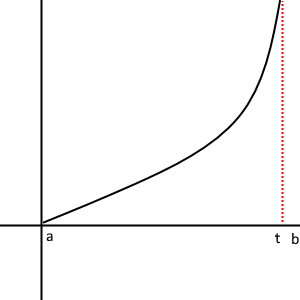
\includegraphics[scale=0.5]{resources/infityFunctionUnormalIntegral.png}

  $\definiteIntegral{b}{a}\defFunction{x}dx = \limNormal{t \to b^-}\definiteIntegral{t}{a}\defFunction{x}dx$

  或者是设a为瑕点:

  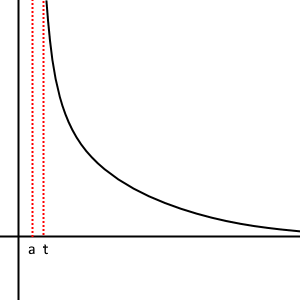
\includegraphics[scale=0.5]{resources/infityFunctionUnormalIntegral2.png}

  $\definiteIntegral{b}{a}\defFunction{x}dx = \limNormal{t \to a^+}\definiteIntegral{b}{t}\defFunction{x}dx$

  或者以上两者情况合一,设c为瑕点将其拆分:

  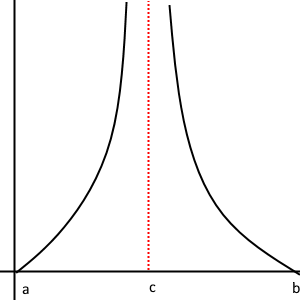
\includegraphics{resources/infityFunctionUnormalIntegral3.png}

  $\definiteIntegral{b}{a}\defFunction{x}dx = \definiteIntegral{c}{a}\defFunction{x}dx + \definiteIntegral{b}{c}\defFunction{x}dx$

  然后按照上方两个情况分别求解。

  依然可以使用牛-莱公式。

  瑕积分换元需要为单调函数,不论增减性。

}%无界函数反常积分

\subsubsection{gamma函数}{
$\varGamma(s) = \definiteIntegral{+\infty}{0}e^{-x}x^{s-1}dx, (s > 0)$

gamma函数的特点就是:

$\varGamma(s + 1) = s\varGamma(s), \varGamma(1) = 1$

因此:

$\varGamma(n+1) = n!$

}%gamma函数结尾

}%反常积分结尾

\subsection{无穷级数}{

\subsubsection{泰勒公式/泰勒级数/展开}{
泰勒级数表示:当知道某点$x = a$的情况时,就能知道$a$点附近的函数是怎样的。

$x$在$a$点附近,最为粗略的估计就是$\defFunction{x} \approx \defFunction{a}$

然后才是修正项:$\fDerivative{a}(x - a)$,这是斜率乘以距离,最终得到的就是高度。相当于沿切线前进。

还有一项表示弯曲:$\frac{1}{2}\fint\doubleDerivative(a)(x - a)^2$,他是斜率的斜率,变化率的变化率。

但后面还有更多项,直接写出通项公式如何?

泰勒级数通项公式:$\defFunction{x} = \upDownSum{\infty}{n = 1}\frac{1}{n!}\fint\aLotDerivative{n - 1}(x - a)^{n - 1}$,0阶导指的是原函数,a是x附近的点。

还有泰勒公式:表示的不是一个函数的幂级数形式而是对于某个函数的近似,形式与泰勒级数通项公式类似。

泰勒公式:$\defFunction{x} = \defFunction{a} + \fDerivative{a}(x - a) + \frac{1}{2!}\fint\doubleDerivative(a)(x - a)^2 + ... + \frac{1}{n!}\fint\aLotDerivative{n}(x - a)^n + R_n(x)$。

$R_n(x)$是余项,表示误差,是$(x - a)^n$的高阶无穷小$O((x - a)^n)$。根据中值定理可得$R_n(x) = \frac{1}{(n + 1)!}\fint\aLotDerivative{n + 1}(\xi)(x - a)^{n+1}$,其中$a \leq \xi \leq x$,意思是$\xi$介于$a$和$x$之间。

当泰勒公式在$a = 0$处展开时就称为麦克劳林公式。

麦克劳林公式:当$a = 0, \defFunction{x} = \defFunction{0} + \frac{1}{1!}\fDerivative{0}x + \frac{1}{2!}\fint\doubleDerivative(0)x^2 + ... + \frac{1}{(n + 1)!}\fint\aLotDerivative{n + 1}(\theta x)x^{n+1}$,其中$0 < \theta < 1$

}%泰勒公式/泰勒级数/展开结尾

}%无穷级数结尾

\subsection{微分方程}{
微分方程是一种描述世界的好手段,当描述某个东西随时间的微小变化比起描述这个物体整体的变化更方便的时候就会使用微分方程。

\subsubsection{一阶线性微分方程}{
  形式$\frac{dy}{dx} + p(x)y = Q(x)$

  有以下几种情况:
  \begin{enumerate}
    \item $Q(x) = 0\ \to$齐次方程,则$\frac{dy}{dx} = -p(x)y\ \to \ \frac{dy}{y} = -p(x)dx$,然后两边求积分,从而得出:$y = e^{-\int p(x)dx}e^{\mathConstant_1} = C \cdot e^{-\int p(x)dx}$
    \item $\frac{dy}{dx} + p(x)y = Q(x), Q(x) \neq 0$,也就是非齐次方程。设$y = ue^{-\int p(x)dx, u}$是未知量。然后把$y$代入:\\ $u\derivative e^{-\int p(x)dx} - ue^{-\int p(x)dx} + p(x)u^{e}-\int p(x)dx = Q(x)$,从而推出:$u\derivative e^{-\int p(x)dx} = Q(x)$,并且由$u\derivative = Q(X)e^{\int p(x)dx}$从而推出:$\int Q(x)e^{\int p(x)dx}dx + \mathConstant$。将以上带入,得出:$y = e^{-\int p(x)dx}\cdot(\int Q(x)e^{\int p(x)dx}dx + \mathConstant)$
  \end{enumerate}

  注:一个非齐次线性微分方程的通解等于对应的齐次微分方程的通解与非齐次微分方程的一个特解之和。

}%一阶线性微分方程结尾

\subsubsection{*有疑惑/错误\ 伯努利方程}{
  $\frac{dy}{dx} + p(x)y = Q(x)y^n$。当$n = 0$时,此式为齐次方程,当$n = 1$,为一阶线性微分方程。当$n$不等于0也不等于1时:$y^{-n}\frac{dy}{dx} + p(x)y^{1-n} = Q(x)$。将$y^{1-n}$记作$z$,于是得到$\frac{dz}{dx} = (1-n)y^{-n}\frac{dy}{dx},\frac{1}{1-n}\frac{dz}{dx} + p(x)z = Q(x)$,再变形得到:$\frac{dz}{dx} + (1-n)p(x)z = (1-n)Q(x)$。然后两边求$y$,左边不要带入。

}%伯努利方程结尾

\subsubsection{可降阶高阶微分方程}{
  有以下几种情况:

  \begin{enumerate}
    \item $y^{(n)} = \defFunction{x}$,于是两边不断求积分进行降阶:$y^{n-1} = \int \defFunction{x}dx + \mathConstant$
    \item $y\doubleDerivative = \defFunction{x,y\derivative}$,设$y\derivative = p,y\doubleDerivative = p\derivative$,则$p\derivative = \defFunction{x,p}$。然后再进行回代。
    \item $y\doubleDerivative = \defFunction{y,y\derivative}$,同样的,令$y\derivative = p, y\doubleDerivative = \frac{dp}{dx} = \frac{dp}{dy}\cdot\frac{dy}{dx} = p\frac{dp}{dy}$,于是$p\frac{dp}{dy} = \defFunction{y,p}$
  \end{enumerate}

}%可降阶高阶微分方程结尾

\subsubsection{常系数齐次线性微分方程}{
  例:$y\doubleDerivative + py\derivative + qy = 0$

  先找出特征方程:$r^2 + pr + q = 0$,即:设$r = p\derivative,r^2 = \doubleDerivative$。

  有以下三种情况:
  \begin{enumerate}
    \item $\Delta = b^2 - 4ac = p^2 - 4q > 0,r_1 = \frac{-p + \sqrt{p^2 - 4q}}{2}, r_2 = \frac{-p - \sqrt{p^2 - 4q}}{2}$
    \item $\Delta = b^2 - 4ac = p^2 - 4q = 0,r_1 = r_2 = \frac{-p}{2}$
    \item {$\Delta = b^2 - 4ac = p^2 - 4q < 0,r_1 = \alpha + \beta_i, r_2 = \alpha - \beta_i$,可扩写成以下三种形式:

          \begin{enumerate}
            \item $y = \mathConstant_1e^{r_1x} + \mathConstant_2e^{r_2x}$($\mathConstant_1,\mathConstant_2$为任意常数)
            \item $y = (\mathConstant_1 + \mathConstant_2)e^{r_1x}$
            \item $y = e^{\alpha x}(\mathConstant_1\cos\beta + \mathConstant_2\sin\beta)$
          \end{enumerate}
          }
  \end{enumerate}

}%常系数其次线性微分方程结尾

\subsubsection{关于运动的微分方程/线性常系数微分方程}{
开门见山,先提出此公式再进行分析。

$m\frac{d^2y}{dt^2} + 2r\frac{dy}{dt} + ky = 0$

很明显,这是个二阶常系数线性微分方程,二阶指的是它最多求了2次导。线性、这意味着他可以是个抽象的向量,他能被线性代数的方式所表示(见4.1.2-关于抽象向量空间)。至于“常系数”,这意味着它的系数都是常数。

先分析这个方程的退化形式。

1、设$m = 0, r = 1/2, \frac{dy}{dt} = ay$

很明显:这意味着函数求导后是它自身的倍数,这暗示着原函数是个指数函数。不难猜到:原函数可以为$y = e^{at}$。但这样还不够。仔细想想:如果e的前面有系数,求导后也依然还是原函数的倍数,所以通解应该是$y = ce^{at}$。

2、设 $r = 0, \frac{d^2y}{dt^2} = -\omega^2y$,其中$\omega$是$\frac{k}{m}$。

这又意味着什么?这意味着:原函数求二次导后是负数倍的他自己,在实数范围内(毕竟一涉及$i$事情就麻烦了起来,不过如果包含虚数的范围倒也是一件合理的事情,设$y=e^{kx},y\doubleDerivative = k^{2}e^{kx}$,如果要使这个二阶导符合条件很明显$k$应该是$i$,而欧拉公式的完整写法是:$e^{ix} = \cos x + i\sin x$)符合这个条件的就这两个函数:$\sin\omega t$和$\cos\omega t$,那么这两个函数就是解集的“基向量/基础解系”,通过这两个函数的线性组合就可以得出所有符合条件的原函数,因此通解写作$y = C\cos\omega t + D\sin\omega t$

3、设$m = 0, r = 0, \frac{dy}{dt} = 0$

这更明显,$y = C + Dt$。(y是个函数,表示位置)

那么回到那个方程:这个方程在很多领域都是很常见的。这个方程能表示一切振动。(比如弹簧,钟表,摆动...)通过选择不同的系数,可以建立各种最简洁的基础模型。

那么以弹簧为例来讲解。例子中$t$表示时间(这就是为什么不用x):

实际上,在这种模型中,常有$r = 0$。那么取$ r = 0$的情况。

有牛顿定律:$F = ma$,m就是质量,a则是加速度,也就是二阶导,因此改写成二阶导形式:$F = m\frac{d^2y}{dt^2}$(不考虑质量损失)

弹簧是悬空拉着一个小滑块的。y的正方向是向下,他表示弹簧的位移,当y是正的时候,弹簧有向上拉的力,而弹簧的力与$y$成正比,比例则是常数$k$。当y很大的时候弹簧被拉的很长,向上拉的力在往上拉,写作$F = -ky = m\frac{d^2y}{dt^2}$其中F表示拉力,负号是因为力的方向与y相反(胡克定理)。经过变形得到:$m\frac{d^2y}{dt^2} + ky = 0$。非常眼熟。

$r = 0$,$r$表示的是阻力,可以是空气阻力也可以是磁力等等,但他就是我们没法制作永动机的原因,不过现在是假想环境,所以设他为0,那么弹簧就会是一根永不停息的、上下振动的弹簧。就如同上面分析的结果,他沿着{\bfseries 正弦和余弦}振动。而常数$C$与$D$则取决于初始状态。

回想一下,$-ky = m\frac{d^2y}{dt^2}$,将两边同除以$m$,负号移走,于是得到$\omega^2$而$\omega^2 = \frac{k}{m}$。

这种情况很简单,只有$\sin , \cos$。接下来,来一点阻力。

$my\doubleDerivative + 2ry\derivative + ky = 0$

现在,对于任意$m,r,k$。想要求解此方程,很棒的是指数函数可以求出正确答案。

核心思想是尝试指数函数$y = e^{\lambda t}$,$\lambda$指的是特征函数。(用$\lambda$而不用$C$的原因可以看4.1.1-什么是线性变换。)将这个代入方程,并求出合适的$\lambda$。何不先从常数项开始?

很容易看出常数项是$ke^{\lambda t}$

而一阶导呢?有$2r$乘以$y = e^{\lambda t}$的导数,只需要将导数代入方程。

一阶项是$2r\lambda e^{\lambda t}$

到二阶导,同理。

二阶项就是$m\lambda^2e^{\lambda t}$

写出完整的形态:$m\lambda^2e^{\lambda t} + 2r\lambda e^{\lambda t} + ke^{\lambda t} = 0$

消掉公因式$e^{\lambda t}$,他显然不是0,可以消掉。结果就是$m\lambda^2 + \lambda + k= 0$

这个方程只不过是个普通的二次方程,随随便便就能解出来。二次方程理应有两个解。因此$e^{\lambda_1 t}$和$e^{\lambda_2 t}$都是方程的解

回忆一下公式,$\lambda = \frac{-r \pm \sqrt{r^2 - km}}{m}$

引入一些数字,$1y\doubleDerivative + 6y\derivative + 8y = 0$。计算$\lambda$

$\lambda^2 + 6\lambda + 8 = 0$

$\lambda_1 = -2, \lambda_2 = -4$

解是多少呢?$y(t) = Ce^{-2t} + De^{-4t}$

两个$\lambda$都在指数中,然后得解

注意:$\lambda$可能解出复数,可以照样用,但也可以写成另一种形式——利用欧拉公式的美妙性质。

$e^{it} = \cos t + i\sin t$

(欧拉第二天意识到$-i$也有公式)

$e^{-it} = \cos t -i\sin t$

让我们直接跳到结果:

$e^{(x \pm ki)t} = e^{xt}\cdot(\cos(t\cdot n) \pm i\sin(t\cdot n))$

另外,当两个$\lambda$相同(出现重根)的时候,方程的解一个是$e^{\lambda t}$另一个是$te^{\lambda t}$,经过验算会发现最后消掉了一部分,得到的是正常的结果。

所以结论就是:线性常系数微分方程只要通过$e^{\lambda t}$就能解决。
}%关于运动的微分方程结尾

\subsubsection{关于增长的微分方程/非线性微分方程/偏微分方程剧透}{
  从线性的开始。

  最简单的:$\frac{dy}{dt} = cy$, 给予了初始条件$y(0)$

  即增长率与自身成正比。很明显的这是呈指数形式的增长,解应该是$y(t) = y(0)e^{ct}$

  看下一个方程,依然是线性的:$\frac{dy}{dt} = cy + s$,$s$表示source,可以用银行存钱来描述:前一项是每天的利息,后一项的每天存入的金额。
  这就是右侧带有常数项的线性微分方程了。事实上甚至能拿现有的知识来解决它:$\frac{dy}{dt} = cy + s = c(y + \frac{s}{c}) = \frac{d(y + \frac{s}{c})}{dt}$, 其中$\frac{s}{c}$是常数,所以可以任意加减而不影响求导结果。随后观察整体,会发现与第一个例子几乎相同,唯一不同的就是多了个$\frac{s}{c}$函数依然以增长率c增长。从0处的y值加上$\frac{s}{c}$开始。

  所以,结论是:$y(t) + \frac{s}{c} = (y(0) + \frac{s}{c})e^{ct}$。这就是该微分方程的快速版解答了。将常数丢到右边,就是一个标准的形式。

  所以线性方程(不只是线性微分方程)的解$y(t) = y_{particular}(t) + y_{another\ solution\ with\ a\ right\ side\ 0}(t)$。用人话说就是:线性方程的解总是自身的某个特解加上另一个右侧等于0的方程的解。

  也就是说如果要求$\frac{dy}{dt} = cy + s$的解,那么首先求一个特解(也就是任一个满足方程的函数),能找到的最简单的函数就是常函数。想要常数满足方程,常熟的常数必然为0,而且c乘以此常数加s也应该为0。也就是$cy + s = 0,\ cy = -s, \ y = -\frac{s}{y}$。这就是一个特解了。

  那么“一个右侧为0的方程的解”是什么意思?将s擦去,使得$\frac{dy}{dt} = cy$,保留含有y的,去掉常数项,使得右侧为0。也就是$y\derivative - cy = 0$。书本上喜欢称之为:齐次方程。也就是第一个例子。

  那么齐次方程的解是什么呢?$\frac{dy}{dt} = cy$的解含有$e^{ct}$以及任意常数$A$,也就是$Ae^{ct}$,任意$Ae^{ct}$都能满足这个简单的方程。

  所以整个方程的解就是$-\frac{s}{c} + Ae^{ct}$A是任意常数。不过当然,如果有初始条件就能特定一个。只需要设$t = 0$,就能解出$A$,在这里$A = y(0) + \frac{s}{c}$。在上面也算出来了。

  不过线性的已经没啥意思了,来点线性的。非线性的微分方程很有趣,也可以表示很多东西,比如:人口的增长。

  关于人口增长函数$P(t)$,用什么微分方程描述比较合理?

  $\frac{dP}{dt} = cP - sP^2$。其中c表示增长率。同样的,有出生也会有死亡,所以需要一个减速项,因为人口增长不可能这么快。也就是s。这在一定程度上反映了人口之间的相互作用。(事实上这种公式在其他领域也有很多用途)

  在这个公式中$p^2$表示人口之间的相互拥挤造成的影响,因此s是个很小的数,比如十亿分之一。

  下面要解这个方程了。

  不过对于非线性方程,目前(正在阅读的你,或者是我自己复习?)暂时没有现成的工具,需要更多的微积分知识。但是只要方法正确,就能解出来的。

  先展示解吧:首先,如果一开始一个人都没有,那么就始终为0。$P = 0$,常数解,很无趣。还有一种情况,很重要的情况,这种情况下导数也为0。

  假设导数为0,将会得到一个特殊的特解,他不会变化。也就是当导数为0时,那么$cP = sP^2$。可以约掉一个P,也就是$P = \frac{C}{S}$。此时,增长和减少将会相互抵消,成为无法逾越的上限。

  那么来看看真实情况下的解,不过为何不先看看图呢?:

  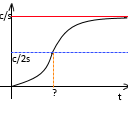
\includegraphics{resources/nonLinearDifferencialEquation_HumanGrow.png}

  其中$\frac{c}{s}$称为稳态,到了这里就会保持稳定,不会改变了。不过其实到不了哪里,只会一直接近而已。这就是这个式子所代表的人口曲线了。

  那么就是解方程的环节了。有很多方法,先试试一个好使的:尝试$y = \frac{1}{P}$。然后尝试把整个方程写成y的形式。这是解这个方程的技巧,而解非线性方程常常需要一些技巧。

  看看这个方程长啥样子:$\frac{dy}{dt} = -\frac{\frac{dP}{dt}}{P^2}$而$\frac{dP}{dt}$是已知的,所以将他代进来,得到$-\frac{cP - sP^2}{P^2}$。将负号写进去,得到一个s:$s - \frac{c}{P}$。查看前面的推导能发现:$\frac{1}{p} = y$。所以得到$s - cy$。于是$\frac{dy}{dt}$变成了线性的,它还含有资源项s,而增长率项还含有一个-c。也许仔细想想为什么

  那么写出y的解:$y(t) - \frac{s}{c} = (y(0) - \frac{s}{c})e^{-ct}$这就是y的解。$y = \frac{1}{P}$,接下来就是要回代了:

  $\frac{1}{P(t)} - \frac{s}{c} = (\frac{1}{P(0)} - \frac{s}{c})e^{-ct}$,接下来的一堆化简就不写了。

  这种模型称为logistic方程(只是为了提一下)

  接下来再来一个有意思的方程:捕食者与猎物的方程:

  这里有两个未知数:猎物——记作$v$,捕食者——记作$u$,表示的都是两者的总数。如果猎物不够,捕食者就会减少。捕食者减少,猎物就会增加。因此这里有正的$u \cdot v$

  这是公式:

  前面有个$-cu$,表示没有食物的情况,捕食者将会慢慢灭绝。

  但如果猎物存在,那么资源项就会正比于$uv$。

  所以$\frac{du}{dt} = -cu + suv$

  那么$\frac{dv}{dt}$呢?情况大不相同。他们被捕食,因此有$-Suv$,同时也有正的增长率$Cv$

  那么这就是一个模型了。剧透一下:这玩意叫偏微分方程(Partical Differential Equation),简称PDE,他比常微分方程(Ordinary Differential Equation, ODE)包含了更多的信息。也更难解。

}%关于增长的微分方程结尾

}%微分方程结尾

}%微积分结尾

\section{高等代数/线性代数}{
\subsection{定义、解释、前言}{
\subsubsection{什么是线性变换}{
  什么是线性变换?线性变换是变换的一种,是操纵抽象的向量空间的手段,通过线性变换可以将空间进行放缩与变形。
  所谓的“线性”意味着这类变换满足以下两个性质:

  \begin{enumerate}
    \item 齐次性:$L(\mathbf{C}\vec{v}) = \mathbf{C}L(\vec{v})$
    \item 可加性:$L(\vec{u}+\vec{v}) = L(\vec{u})+L(\vec{v})$
  \end{enumerate}

  其实所谓的线性通常指的就是这回事,而满足线性也通常暗示着某种可能——用矩阵表示对象的可能。
  举个例子,求导就是一种线性运算,它符合以上的两个条件。事实上也并不是只有一次幂的函数可以用线性代数的方法表示。

  正因大部分函数可以表示成矩阵与向量,事实上线性代数的很多概念都在函数中有直接类比,比如:

  \begin{tabular}{c|c}
    \hline
    线性代数中的概念                & 应用于函数时的别名          \\
    \hline
    线性变换(Linear transformation) & 线性算子(Linear operatiors) \\
    点积(Dot products)              & 内积(Inner products)        \\
    特征向量(Eigen vectors)         & 特征函数(Eigen functions)
  \end{tabular}

  可以看出数学中还有很多类似向量的事物。只要所处理对象,具有合理的数乘和加和概念,不管是空间中的箭头、一组数还是函数集合,线性代数中所有关于向量、线性变换和其他的概念都应该适用于它。这些类似向量的事物,它们构成的集合被称为向量空间。这些内容将在“抽象向量空间”章节中讨论
}%线性变换结尾

\subsubsection{关于抽象向量空间}{
为什么要定义这么麻烦的规则?在数学的表达中,我们倾向于得到用普适的概念,{\bfseries而普适的代价就是抽象}。在日常生活中不难发现很多东西都给人一种线性的错觉,事实上那不是错觉,向量也不一定得是箭头或坐标什么的,因此为了规范向量的定义,得到所期望的普适性,抽象出以下规则,这意味着:如果要将一类对象称为向量并且对其运用线性代数的知识,则必须满足以下条件。

(也可以称这堆玩意为向量加法和数乘的规则):
\begin{enumerate}
  \item $\vec{u} + (\vec{v} + \vec{w}) = (\vec{u} + \vec{v}) + \vec{w}$
  \item $\vec{v} + \vec{w} = \vec{w} + \vec{v}$
  \item 存在一个$\vec{0}$使得$\vec{0} + \vec{v} = \vec{v}$,这应该对于所有$\vec{v}$都成立。
  \item 对于所有的$\vec{v}$,都存在$-\vec{v}$,使得$\vec{v} + (-\vec{v}) = \vec{0}$
  \item $a(b\vec{v}) = (ab)\vec{v}$
  \item $1\vec{v} = \vec{v}$
  \item $a(\vec{v} + \vec{w}) = a\vec{v} + a\vec{w}$
  \item $(a + b)\vec{v} = a\vec{v} + b\vec{v}$
\end{enumerate}

在新定义的向量空间中应用线性代数的结论之前,需要验证它的定义是否满足以上要求。

如果要让已经建立好的线代理论和概念适用于一个空间,那么必须满足这8条公理。这8条公理保证新定义的向量,其加法和数乘符合你一直接受的状态。

那么,有了这些明确的规则,就可以在任何{\bfseries符合这些规则}的抽象的向量空间中使用线性代数了。
}%关于抽象向量空间结尾

}%定义、解释、前言结尾

}%高等代数/线性代数结尾

\section{数论}{

 }%数论结尾

\section{场论}{

 }%场论结尾

\section{群论}{

 }%群论结尾

\section{矩阵论}{

 }%矩阵论结尾

}%数学篇结尾

\chapter{计算机科学}{

  \section{编程}{


   }%编程结尾

  \section{网络安全}{


   }%网络安全结尾

  \section{重要技术}{

    \subsection{计算机图形学}{
      注:本章中向量默认为列向量。

      \subsubsection{对于线性代数部分的补充与扩展}{

        在计算机图形学中线性代数的主要作用是操纵与计算空间中对象的变化。由此衍生出了一些特殊的东西。

        同时有一部分重要的常用基础内容放在了数学篇中的空间解析几何部分。

        \begin{enumerate}
          \item {向量叉乘的对偶矩阵:
                $$\vec{a} \times \vec{b}
                  =
                  \left[\begin{matrix}
                      y_az_b - y_bz_a \\
                      z_ax_b - x_az_b \\
                      x_ay_b - y_ax_b
                    \end{matrix}\right]
                  =
                  A * \vec{b}
                  =
                  \left[\begin{matrix}
                      0    & -z_a & y_a  \\
                      z_a  & 0    & -x_a \\
                      -y_a & x_a  & 0
                    \end{matrix}\right]
                  \left[\begin{array}{c}
                      x_b \\
                      y_b \\
                      z_b
                    \end{array}
                    \right]
                $$
                }
          \item 非满秩矩阵意味着将空间变换到了更低的维度。
          \item 特征向量是指在进行了矩阵所代表的线性变换后方向没改变向量,特征值则是指特征向量的缩放倍数。
          \item 逆矩阵所代表的变换成为逆变换,是原矩阵所代表的变换的反向操作,一个矩阵乘以他的逆矩阵是单位阵,这从几何上的直观理解就是什么都没做,两次操作互相抵消了。
        \end{enumerate}
      }

      \subsubsection{变换}{
        变换按照作用对象可以分为:
        \begin{enumerate}
          \item Modeling 模型变换
          \item Viewing 视角变换
        \end{enumerate}

        按照作用效果可以分为:
        \begin{enumerate}
          \item scale 缩放变换
          \item rotate 旋转变换
          \item shear 剪切变换
        \end{enumerate}

        如同3b1b的观点,将目标空间看作矩阵的列空间。而矩阵每一列都对应了列空间中的一个基向量,拿2维空间举例:
        $$\left[\begin{matrix}
              1 & 0 \\
              0 & 1
            \end{matrix}\right]$$

        假设第一列代表了$x$轴的单位向量$i$,则第二列代表了$y$轴的单位向量$j$

        因此,对矩阵进行操作就相当于对矩阵所代表的空间进行操作。

        例如:$$\left[\begin{matrix}
              2 & 1 \\
              1 & 2
            \end{matrix}\right]$$

        这个矩阵就代表着将单位向量$i$移动到了坐标$(2,1)$,将单位向量$j$移动到了坐标$(1,2)$。整个二维空间都是由这两个单位向量所张成的。随着单位向量的移动,整个空间也就随之而变形。这种操作被称为变换。
        其中一类最简单的变换称为线性变换,在线性代数篇中已有了详细解释。

        旋转矩阵的表示原理如下:

        先看看二维:

        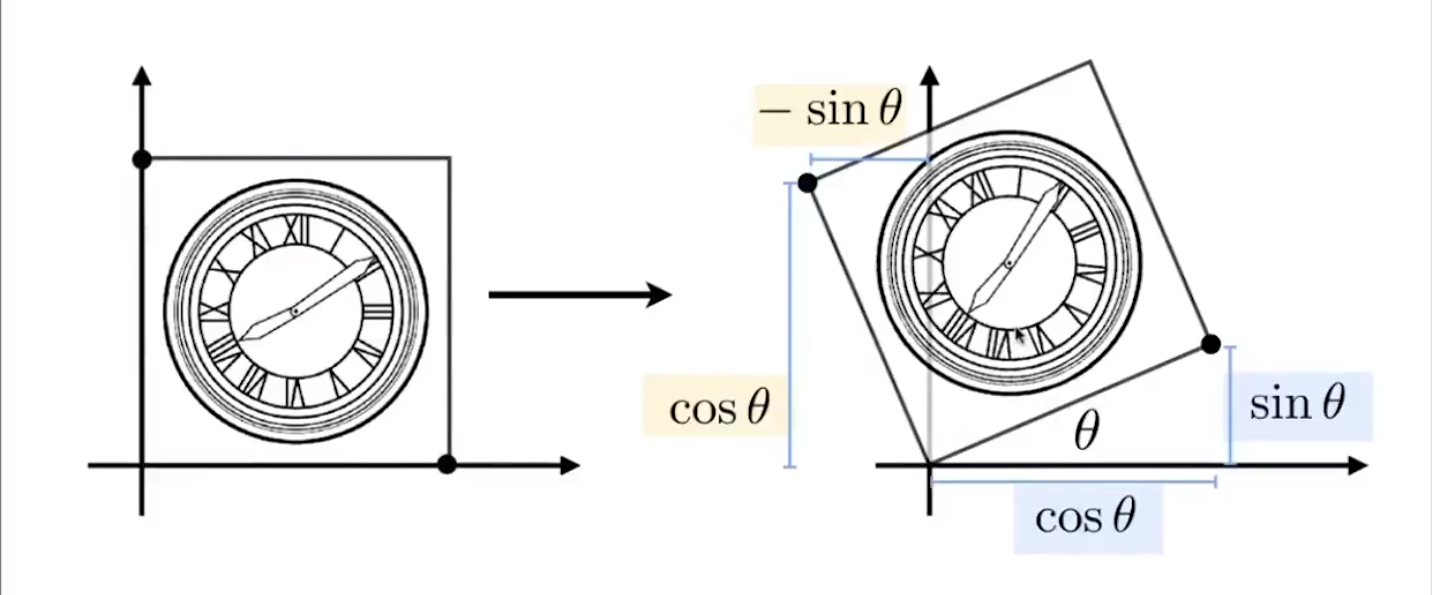
\includegraphics[scale=0.25]{resources/rotateMatrixGraphics.png}

        因此二维的旋转矩阵$$R_\theta = \left[\begin{matrix}
              \cos\theta & -\sin\theta \\
              \sin\theta & \cos\theta
            \end{matrix}\right]$$

      }%变换结尾

      \subsubsection{齐次坐标}{
        由于单纯的线性变换并不能让对象动起来,依然只能在原点操作,所以需要齐次坐标表示空间上的位移。

        如下图:

        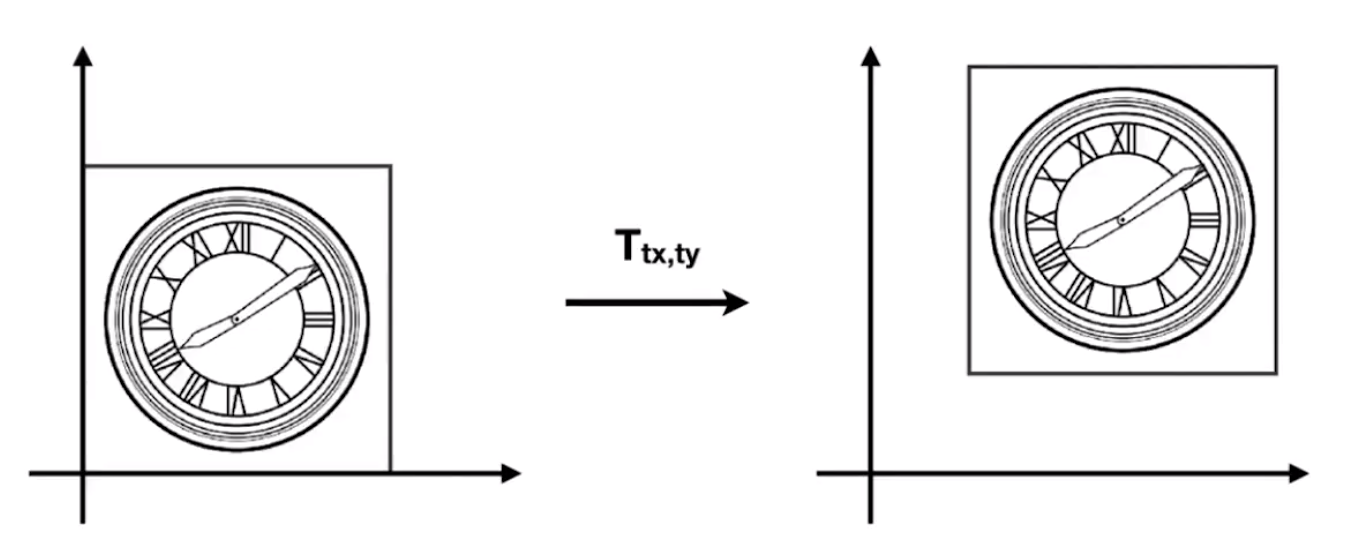
\includegraphics[scale=0.25]{resources/homogeneous_coordinates.png}

        用$x\prime$和$y\prime$来表示变换后的坐标,公式为:

        $x\prime = x + t_x$

        $y\prime = y + t_y$

        仔细思考一下发现似乎并不能写成矩阵$A\vec{x} = \vec{b}$的形式。

        事实上应该写成这样:
        $$
          \left[\begin{array}{c}
              x\prime \\
              y\prime
            \end{array}\right]
          =
          \left[\begin{matrix}
              a & b \\
              c & d
            \end{matrix}\right]
          \left[\begin{array}{c}
              x \\
              y
            \end{array}\right]
          +
          \left[\begin{array}{c}
              t_x \\
              t_y
            \end{array}\right]
        $$

        因此平移变换不属于线性变换。但是人们不想要特殊情况,于是引入了齐次坐标:

        还是拿二维的情况举例,增加一个维度,将二维的点表示为:
        $$\left[\begin{array}{ccc}
              x & y & 1
            \end{array}\right]^T$$

        将二维向量表示为:
        $$\left[\begin{array}{ccc}
              x & y & 0
            \end{array}\right]^T$$

        也就是说:再多增加一个维度用于说明表示的是一个点还是一个向量,这是因为向量具有平移不变性,不管怎么移动表示的始终是一个方向。

        齐次坐标的好处就在这里,它是这么用的:

        $$\left[\begin{array}{c}
              x\prime \\
              y\prime \\
              w\prime
            \end{array}\right]
          =
          \left[\begin{matrix}
              1 & 0 & t_x \\
              0 & 1 & t_y \\
              0 & 0 & 1
            \end{matrix}\right]
          \cdot
          \left[\begin{array}{c}
              x \\
              y \\
              1
            \end{array}\right]
          =
          \left[\begin{array}{c}
              x + t_x \\
              y + t_y \\
              1
            \end{array}\right]
        $$

        更直观一点:可以这么理解:
        \begin{itemize}
          \item vector + vector = vector 向量相加还是向量 $0 + 0 = 0$
          \item point - point = vector 两点相减得到向量 $1 - 1 = 0$
          \item point + vector = point 一个点加一个向量结果是一个点 $0 + 1 = 1$
          \item point + point = 两个点的中点 $1 + 1 = 2$,原因见扩充定义。
        \end{itemize}
        扩充定义如下:
        $$\left[\begin{array}{c}
              x \\
              y \\
              w
            \end{array}\right]$$是二维的点,可化简为:$$\left[\begin{array}{c}
              x \\
              y \\
              w
            \end{array}\right]\cdot\frac{1}{w} = \left[\begin{array}{c}
              \frac{x}{w} \\
              \frac{y}{w} \\
              1
            \end{array}\right]$$

        {\bfseries于是总结,给出以下下定义:}\\\\\indent
        仿射变换(Affine transformation) = 线性变换(Linear transformation) + 位移(transformation)

        即:
        $$\left[\begin{array}{c}
              x\prime \\
              y\prime
            \end{array}\right]
          =
          \left[\begin{matrix}
              a & b \\
              c & d
            \end{matrix}\right]
          \cdot
          \left[\begin{array}{c}
              x \\
              y
            \end{array}\right]
          +
          \left[\begin{array}{c}
              t_x \\
              t_y
            \end{array}\right]$$

        都可以写成齐次坐标(homogeneous coordinates)的形式

        即:
        $$\left[\begin{array}{c}
              x\prime \\
              y\prime \\
              1
            \end{array}\right]
          =
          \left[\begin{matrix}
              a & b & t_x \\
              c & d & t_y \\
              0 & 0 & 1
            \end{matrix}\right]
          \cdot
          \left[\begin{array}{c}
              x \\
              y \\
              1
            \end{array}\right]$$

        {\bfseries不如直接将其他操作的齐次坐标形式补全吧?}
        \begin{itemize}
          \item 缩放(scale) : $$S(s_x, s_y) = \left[\begin{matrix}
                      s_x & 0   & 0 \\
                      0   & s_y & 0 \\
                      0   & 0   & 0
                    \end{matrix}\right]$$
          \item 旋转(rotation) : $$R(\alpha) = \left[\begin{matrix}
                      \cos\alpha & -\sin\alpha & 0 \\
                      \sin\alpha & \cos\alpha  & 0 \\
                      0          & 0           & 1
                    \end{matrix}\right]$$
          \item 平移(translation) : $$T(t_x, t_y) = \left[\begin{matrix}
                      1 & 0 & t_x \\
                      0 & 1 & t_y \\
                      0 & 0 & 1
                    \end{matrix}\right]$$
        \end{itemize}

      }%齐次坐标结尾

      \subsubsection{组合变换}{
        可以通过组合各个基础变换以形成复杂的变换效果。

        组合方法为对应矩阵按照顺序从右向左做乘法。

        大部分时候组合顺序至关重要。

      }%组合变换结尾

      \subsubsection{三维变换}{
        以上结论都可以用于三维,推而广之:\\

        齐次坐标:\begin{itemize}
          \item 三维点:$$\left[\begin{array}{c}
                      x \\
                      y \\
                      z \\
                      1
                    \end{array}\right]$$
          \item 三维向量:$$\left[\begin{array}{c}
                      x \\
                      y \\
                      z \\
                      0
                    \end{array}\right]$$
        \end{itemize}

        $\left[x\ y\ z\ w\right]^T$,当$w$不等于$1$他所表示的三维的点其实是(第四个维度已略去):
        $$\left[\begin{array}{c}
              \frac{x}{w} \\
              \frac{y}{w} \\
              \frac{z}{w} \\
            \end{array}\right]$$

        同样的,三维空间中齐次坐标描述的仿射变换的矩阵是$4 \times 4$的:
        $$\left[\begin{array}{c}
              x\prime \\
              y\prime \\
              z\prime \\
              1
            \end{array}\right]
          =
          \left[\begin{matrix}
              a & b & c & t_x \\
              d & e & f & t_y \\
              g & h & i & t_z \\
              0 & 0 & 0 & 1
            \end{matrix}\right]
          \cdot
          \left[\begin{array}{c}
              x \\
              y \\
              z \\
              1
            \end{array}\right]$$
      }

    }%计算机图形学结尾

   }%重要技术结尾

  \section{硬件}{

   }%硬件结尾

  \section{网络通信}{

   }%网络通信结尾

  \section{科研辅助}{

   }

 }%计算机科学篇结尾
\end{document}